\section{Pulsar Populations and Age}
\label{sec:popAndAge}

\begin{figure}[t!!]
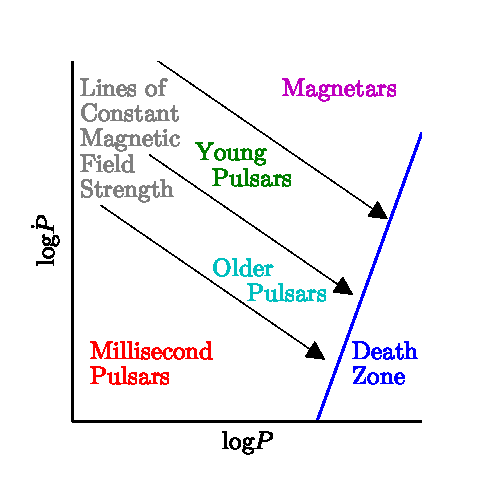
\includegraphics[width=.95\textwidth]{chapters/pulsarAnatomy/figures/ppdot.eps}
\caption[Period-period derivative schematic plot]{
\label{fig:ppdot} Period-period derivative schematic plot.}
\end{figure}

As pulsars age, their rotational period slows due to 
the loss of energy into the pulsar wind. 
Integration of Equation \ref{eq:angFreq} gives the characteristic
age of the pulsar as $t=P/2\dot{P}$
where $n=3$ or equivalently, $P\dot{P}$ is the
constant that relates $\Omega$ and $\dot{\Omega}$.
This relation is based on the assumption 
that the magnetic field
remains constant over time.

Figure~\ref{fig:ppdot} shows a schematic of various
pulsar populations.  Most pulsars start their
life in the upper left corner of the $P$--$\dot{P}$ diagram
and move diagonally downward along lines of constant
magnetic field strength.  Eventually, pulsars enter the ``death zone'' 
where they are not energetic enough to be observed.

In this thesis work, we focus on young pulsars
that are energetic enough to emit in both
radio and $\gamma$-ray wavelengths, allowing
for possible multi-wavelength studies.
Another population of pulsars that 
are energetic enough to emit in the
$\gamma$-rays are the millisecond pulsars
located in lower left corner of Figure~\ref{fig:ppdot}.

While young pulsars are rotation-powered, rotating
through the loss of rotational energy, millisecond
pulsars are accretion powered.  They are ``spun up''
by their companion star.
When the companion star of the neutron star overflows
the Roche lobe, it imparts material and angular momentum
onto the pulsar.  As a result, millisecond pulsar
periods are much faster and more 
precise compared to normal pulsar periods.




